%%% Preamble
\documentclass[paper=letter, fontsize=11pt]{scrartcl}
\usepackage[T1]{fontenc}
\usepackage{fourier}
\usepackage[space]{grffile}
\usepackage[english]{babel}
\usepackage[protrusion=true,expansion=true]{microtype}	
\usepackage{amsmath,amsfonts,amsthm}
\usepackage[pdftex]{graphicx}
\usepackage{url}
\usepackage{graphicx}
\usepackage{listings}
\usepackage{caption}
\usepackage{pdflscape}
\usepackage{amsmath}
\usepackage{subcaption}
\usepackage{float}
\usepackage{comment}
\usepackage{amsmath}
\setcounter{tocdepth}{3}
\usepackage{color}
\definecolor{identifierColor}{rgb}{0.65,0.16,0.16}
\lstset{identifierstyle=\color{identifierColor}}

%%% Custom sectioning (sectsty package)
\usepackage{sectsty}
\allsectionsfont{\centering \normalfont\scshape}

\usepackage[top=1in, bottom=1in, left=1in, right=1in]{geometry}

%%% Custom headers/footers (fancyhdr package)
\usepackage{fancyhdr}
\pagestyle{fancyplain}
\fancyhead{}
\fancyfoot[C]{}
\fancyfoot[R]{\thepage}							% Pagenumbering


\renewcommand{\headrulewidth}{0pt}				% Remove header underlines
\renewcommand{\footrulewidth}{0pt}				% Remove footer underlines
\setlength{\headheight}{13.6pt}


%%% Equation and float numbering
\numberwithin{equation}{section}		% Equationnumbering: section.eq#
\numberwithin{figure}{section}			% Figurenumbering: section.fig#
\numberwithin{table}{section}			% Tablenumbering: section.tab#


%%% Maketitle metadata
\newcommand{\horrule}[1]{\rule{\linewidth}{#1}}
\title{
		\vspace{-1in} 	
		\usefont{OT1}{bch}{b}{n}
		\normalfont \normalsize \textsc{ME/EE Design Capstone 450} \\ [25pt]
		\horrule{0.5pt} \\[0.4cm]
		\huge Design Review I \\
		\horrule{2pt} \\[0.5cm]
}
\author{
        \normalfont 							
        \normalsize
        Edited by: \\
        Sam Li \\ limutian@yahoo.com \\[2pt]
        Sasha Sheng \\ sasha@sashasheng.com\\[2pt]
        Christina Yan \\ yyoucai@umich.edu\\[2pt]
        Siyuan Zhang\\ kevin.zhangsiyuan@gmail.com\\[2pt]
        Wang Zi \\ waziprince@163.com\\ [2pt]
         Sponsored: \\ Dr. Shane Johnson,  shane.johnson@sjtu.edu.cn\\ \vspace{0.5cm}
}

%%% Begin document
\begin{document}
\maketitle
\begin{figure}[H]
    \centering
    
\includegraphics[scale=0.7]{LOGO.png}
\end{figure}
\pagebreak
\tableofcontents
\pagebreak
	
\section{Revised Abstract}	
In this paper, an innovative design for analyzing blood perfusion is presented. Blood perfusion can be detected and
taken as reference of several disease or damage, such as cancer or burn. So far Laser Doppler Imaging (LDI) is a 
common way to give analysis of blood perfusion, and active dynamic thermal (ADT) is an alternative. Both of 
these two methods have their 
limitations. LDI is too expensive, and ADT needs external excitation which can cause pain to patients. The innovative design is to 
investigate the thermal response captured by an IR camera as a result of internal excitation (heart beat), and output an 
integrated picture that shows the blood perfusion. Customer requirements and engineering 
specifications are given to combine this design with real-life demands. Primary concerns for the customers are effectiveness
of the method and the appropriate pricing. Factors such as signal to noise ratio, cost and repeatability of measurements are the
main critical points for engineering specifications. If succesful, 

\section{Problem Description \& Introduction}

Although it`s hard to see under the human skin, it is necessary for evaluating blood perfusion.
A typical use of inspecting blood perfusion is to evaluate burn depth, which is important because wounds of different 
burn depths require different treating methods, ranging from conservative to surgical. Clinical evaluation,
mainly based on visual inspection, only ensures an accurate prognosis in 50-70\% cases \cite{Renkielska}. Histopathological
assessment is an alternative choice. While it provides accurate results, it is invasive and requires taking multiple
burn wound biopsies and incurs a delay of several days while waiting for the result \cite{Renkielska}. It also requires 
experience of doctors. Another current technology to accurately show
blood perfusion condition is Laser Doppler Imaging(LDI) \cite{Pape}. However, it is expensive (one machine costing
about one-half million U.S. dollars) and not widely affordable and accessible.

We are developing a system that is inexpensive, easy to use and provides accurate results in inspecting blood perfusion
for medical purposes. Our system takes infra-red pictures, which after being analysed provides information
about blood perfusion. Previous research works on using active-dynamic infra-red thermal imaging(ADT)
to evaluate perfusion and burn depth have shown that infra-red pictures can provide accurate results in
discriminating burn depths \cite{Renkielska}\cite{Ruminski}. The ADT method applies an external excitation(heat/light) to the wound area, and then uses
infra-red camera to look at thermal transients at the surface of the wound, which can be used to determine
the burn wound depth \cite{Renkielska}\cite{Ruminski}. Our system is different from these infra-red methods mainly in that
we do not use an external excitation source. Using an infra-red camera with higher accuracy, we will be able
to monitor the spontaneous fluctuation of human body temperature, which goes up when the heart pumps blood
to the body, and drops between heart beats. We trigger the infra-red camera to take a series of pictures
when body temperature rises, thus using human heart beat as the internal excitation source. Based on
the same principle as ADT, we expect our method to also provide accurate evaluations of blood perfusion. Our final
set-up is simpler than ADT methods because we do not need external excitation source. This also means less pain
for the patient because we do not stimulate the already wounded area. We also expect lower noise-signal ratio for
our method because we do not have to filter out the unuseful reflection signal, which is noise for the system. In
the ADT method devoted work has to be done to deal with such noise \cite{Ruminski}.
Our result should be more accurate because we operate in a smaller temperature range, which is determined by the
spontaneous fluctuation of human body temperature.

\section{Information Sources}


After literature review, we are able to get the following benchmarking information. Current methods of evaluating burn depth
include clinical evaluation, histopathological assessment and Laser Doppler Imaging. Clinical evaluation is where doctors
assess burn depth visually based on their experience, and it is only accurate 50-70\% of the times \cite{Renkielska}.
Histopathological assessment is the method where multiple burn wound biopsies are taken for evaluation. Although it provides
accurate results, it incurs a delay of several days \cite{Renkielska}. It also relies on experience of doctors. Laser Doppler Imaging(LDI) 
is a method that is accurate and fast \cite{Pape}. However, each LDI machine costs about one-half million U.S. dollars.
Therefore it is not widely affordable and accessible.

\pagebreak
\section{Customer Requirements and Engineering Specifications}
\subsection{Stakeholder Analysis \& Customer Requirements}
There are three parties of customers for our project. There are companies in the medical device and diagnose industry, companies such as Covidien, Johnson \& Johnson, General Electric, Siemens AG, Stryker Corp, etc.\cite{cres1}. Hospitals are also our stakeholders, since it is where the device will be deployed. Patients are our endusers, therefore they are also included as one of our customers.
Our primary stakeholders are medical device provider because we would be selling the device directly to them, however, we place the most emphasis on the need and requirements of the patients. Table~\ref{Patients CR}, Table~\ref{Hospitals CR}, Table~\ref{Medical Devices CR} below are our analysis of customer requirements based on those three kinds.
\begin {table}[H]
\centering
\begin{tabular}{l|p{12cm}}
CR 1 & Primary concern: the effectiveness and accuracy to analyze problems with blood perfusion \\ \hline
CR 2 & Reasonable cost for one time use \\ \hline
CR 3 & Less medical procedures to diagnose \\ \hline
CR4 & non-invasive.
\end{tabular}
\caption{Patient's Requirements}
\label{Patients CR}
\end{table}

\begin {table}[H]
\centering
\begin{tabular}{l|p{12cm}}
CR 1 & Primary concern: all from the table above \\ \hline
CR 2 & Reasonable cost to purchase one machine \\ \hline
CR 3 & User friendly
\end{tabular}
\caption{Hospital's Requirements}
\label{Hospitals CR}
\end {table}

\begin {table}[H]
\centering
\begin{tabular}{l|p{12cm}}
CR 1 & Primary concern: all from the table above \\ \hline
CR 2 & Reasonable cost to manufacture one machine \\ \hline
\end{tabular}
\caption{Medical Device Provider's Requirements}
\label{Medical Devices CR}
\end {table}

Our stakeholders will also include our major design instructors and mentors, however, the house of quality diagram included below will be from the above three tables.

\subsection{QFD Design}
\begin{quotation}
QFD (Quality Function Deployment) is a method to transform user demands into design quality, to deploy the functions forming quality, and to deploy methods for achieving the design quality into subsystems and component parts, and ultimately to specific elements of the manufacturing process.

\hfill --John R. Hauser
\end{quotation}

\begin{figure}[H]
    \centering
	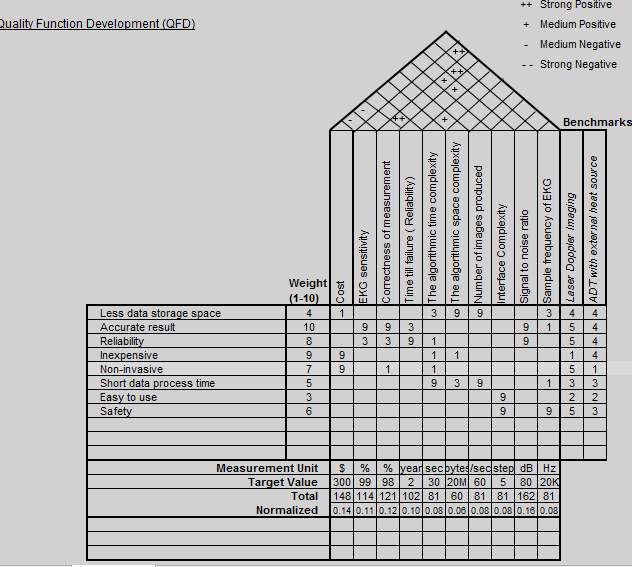
\includegraphics[scale=1]{qfd.png}
	\caption{QFD graph}
\end{figure}

\subsubsection{Determine the weights for Customer Requirements}
Once we got all the customer requirements, we started to rank them based on their importance. As a medical equipment, getting an accurate result is always the first goal. Thus we ranked it first, and then follows Inexpensive, Reliability, Non-invasive, Safety, Short data process time, Less data storage space and Easy to use.

\begin{figure}[H]
    \centering
	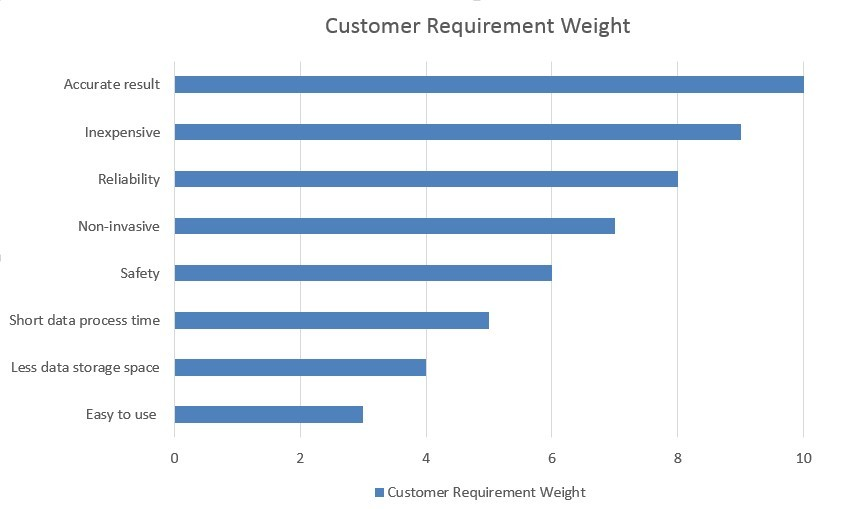
\includegraphics[scale=0.7]{CRweight.jpg}
	\caption{The Weights of Customer Requirements}
\end{figure}
According to this chart, accurate result is our first concern, so we should focus on the design process that can improve the accuracy of our product. Then we need to control the cost and reliability of the product which are the two other main requirements. After that, we would consider design our product to make it non-invasive, safety, short process time, less data storage space and easy to use, which we may have more freedom in making decision. To be clear, safety is important anyway, however in our case, our product is less likely to be unsafe, and so it's just not our main concern. 

\subsubsection{Benchmark the competitions against Customer Requirements}
In our project, we take Laser Doppler Imaging and ADT with external heat source as our benchmarks. Laser Doppler Imaging is highly accurate and reliable but really expensive and need expert to operate, so it gets full scores in accurate result and reliability while gets poor scores in inexpensive and easy to use. As for ADT with external heat source, it's relatively cheap and accurate, however, external heat source may made burned patient suffer more, so it got poor scores in non-invasive and safety.

\subsubsection{Generate Engineering Specifications}
Since we have already analyzed the customer requirements, the next step to develop our QFD is to specify the engineering specifications of our product. Cost was the first characteristic that came to our mind since we didn't have throughout design plan of our product at beginning.  Then we started to find other corresponding engineering specifications. Since the weight of accurate result ranks first in customer requirements, we come up with EKG sensitivity, correctness of measurement, time till failure (Reliability), signal to noise ratio and sample frequency of EKG as relevant characteristics. After that, according to our design procedure, we come up with other engineering specifications, including the algorithmic time complexity, the algorithmic space complexity, Number of images produced, Interface Complexity and sample frequency of EKG.

\subsubsection{Cross Correlate Engineering Specifications}
We want to cross correlate engineering specification because changing one engineering specification can affect others. Take cost as example, if we want to improve the sensitivity of EKG or the correctness of measurement, the cost of our product will increase correspondingly. The increase of cost is negative to us, so we assigned negative to the cross correlate between cost and sensitivity of EKG and correctness of measurement. And specifications like correctness of measurement and signal to noise ratio has positive relationship to each other, so we assigned strong positive between them. Then we fill the rest of correlate as well.

\subsubsection{Correlate Customer Requirements to Engineering Specifications}
Here we come to the most important part of QFD. For each pair of a specification and a requirement, we are supposed to enter correlation value\cite{450}: \\
9 = strongly related \\
3 = somewhat related, where 3 is not a typo \\
1 = weakly related. \\
Take cost as example, we traced back to customer requirements, found that inexpensive and non-invasive were most corresponding to the cost, and less data storage space also had some relative. Thus we assigned inexpensive and non-invasive nine points corresponding to cost, and gave less data storage space a one. This is how we start fill this QFD chart. Then we followed the step to fill rest of chart, keeping in mind the every specification must have a strongly related customer requirement.
\subsubsection{Importance Rating}
After we finished the correlate Customer Requirements to Engineering Specifications part, we can come to the importance rating of specifications. This rating is based on correlation between Customer Requirements to Engineering Specifications, and relative importance is normalized row above. 

\begin{figure}[H]
    \centering
	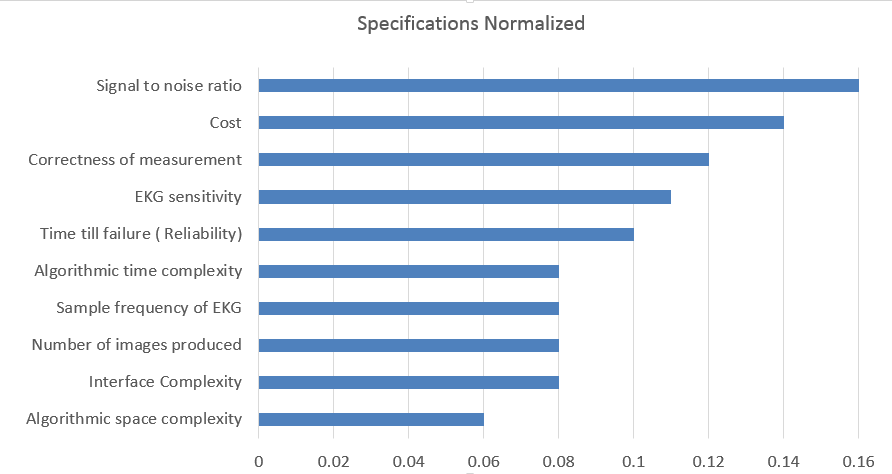
\includegraphics[scale=0.7]{zhentmfan.png}
	\caption{The Engineering Specifications}
\end{figure}

In our case, signal to noise ratio, cost and correctness of measurement are most important specifications on which we should pay most attention. Then follows EKG sensitivity, reliability, sample frequency of EKG and number of images produced. And the algorithmic time complexity and algorithmic space complexity turned out to be less important, where we can have more design freedom.
\subsubsection{Set Targets for Engineering Specifications}
Setting targets for Engineering Specifications that you just come up with is a kind of like brainstorm. We need to search for the present criteria to make our value reasonable, and also ensure its uniqueness to show our innovation. Thus, we set targets for our Engineering Specifications as following:

\begin{figure}[H]
	\centering
	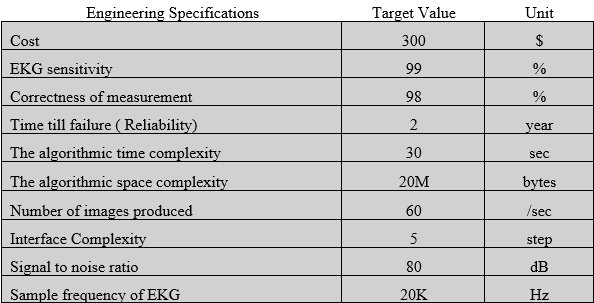
\includegraphics[scale=1]{target.png}
	\caption{The Target Values}
\end{figure}

\subsection{Functional Requirements}
Devices: 
\begin{enumerate}{\alph{enumi}}
	\item EKG, a device we use to trigger the infra-red camera to take a set of samples
	\item Infrared camera
	\item LabVIEW for data acquisition
\end{enumerate}
Below are the sequence of tasks we need to accomplish:
\begin{description}
   \item[Basics - Minimum Viable Product (MVP)] \hspace{1cm}
   	\begin{itemize}
   	\item[\textbf{Task 1}] Literature Research\\
   	\hfill Verification: Have a basic understanding of the current technology and how it compares with what we are doing.
	\item[\textbf{Task 2}] Making the EKG, wiring the circuits\\
	\hfill Verification: Attach the EKG to oscilloscope, and it should give you a graph of the signal. Or LabVIEW program should generate a peak signal to indicate the heart beat, we should be able to see the electrical signal on the graph.
   	\item[\textbf{Task 3}]  EKG should be working, and have a trigger signal once the heart beats.\\
    	\hfill Verification: Same as above, and we should decrease the reaction time and maximize the trigger signal
   	\item[\textbf{Task 4}]  EKG should be able to trigger the IR camera to get a series of images as the data source\\
    	\hfill Verification: LabVIEW program should be able to get a sequence of data, and we should be able to see those images as they are generated.
   	\item[\textbf{Task 5}]  Signal processing to reduce noise\\
   	\hfill Verification: We should be able to observe that the signal to noise value increase
	\item[\textbf{Task 6}] Software algorithm to quickly process the images. \\
   	\hfill Verification: The end result should be one image of blood perfusion that describes the $\delta T$.   
\end{itemize}
  
  \item[Addons] \hspace{1cm}
  	\begin{itemize}
   	\item[\textbf{Task 7}] Improve the sensitivity of EKG device\\
	\hfill Verification: It should collect images faster as soon as it detects the pitch \\
	\item[\textbf{Task 8}] Fast Algorithm: Improve the algorithm to reduce the time complexity and space complexity \\
	\hfill Verification: This can be checked by adopting stress tests.
	\item[\textbf{Task 9}] Fast Processing: Asynchronous processing when the images are generated to reduce processing time.\\
   	\hfill Verification: Processed images and data should be available even when the camera is still taking pictures.
	\end{itemize}
	
  \item[Non-technical requirements]\hspace{1cm}
  	\begin{itemize}
	\item[\textbf{Task 10}] The device should be non-invasive when used on patients. \\
	\hfill Clarification: The device should not apply a heat source to the patients to agitate the injury situation. And it should not require the doctors to perform surgery when making the judgement of the severity of the injury.
	\end{itemize}
\end{description}

\subsection{Non-Functional Requirements}
 \begin{description}
  	\item[Availability/Reliability:]
	The device should be available for most of the time, and it should be reliable to provide an accurate result. However, the patient`s skin color is a major factor that might affect the device`s reliability. Patients with a light skin color will make the device generate more accurate result, since there will be less noise.
	\item[Usability:]
	The device should provide encapsulation of its internal side, so that the medical personnel only need to be able to read from the images and data points to come up with a judgement on the patient`s injury.
	\item[Performance/Speed of the User Experience:]
	Large information back-end data processing. Essentially, we want to be able to do asynchronous programming, and/or threading. The different threads running at the same time. Therefore the speed should not be too slow. The user experience should be improved with a nice interface. Building an interface would be the next thing we do on our list once we have our MVPs and Addons complete.
\end{description}

\section{Project Plan}
The project is basically is divided into four periods. The first is the preparation. During this, we study about the current technology and learn about the software and machines we are going to use.  We have done with this part and have already started the next, generating and converting the heart beat signals from the ECG machine. We have set up the device for collecting the heartbeats and read that from the device to LabVIEW. We are in the process of stabilizing the signal and converting that. The third part is the major body of the project, during which we are going to develop the algorithm to trigger the camera to take multiple pictures and finally combine them into a single image, showing the integrated information to the doctor directly.  The last period we will do the testing. We will have each part works as a whole and hopefully we can contact the local hospital and do some tests in the real cases.
The full view of the gantt chart is included at the end of this document.
\begin{figure}[H]
	\centering
	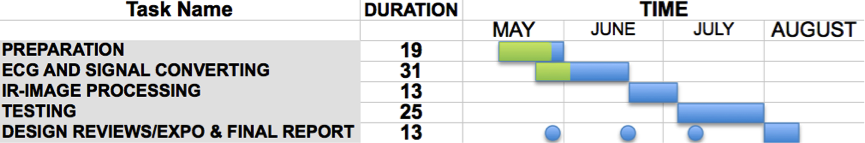
\includegraphics[scale=1]{pjp}
	\caption{Project Plans for major events}
\end{figure}

\section{Conclusions}
\begin{enumerate}
\item Current technology has their own limitations. For LDI machine, it costs up to a million dollars and it is 
hard for LDI to detect other under dark skin abnormalities. For ADT imaging, external excitation makes patients
feel more painful and lead to more noise disrupting the result. \\
\item Our design is accurate, non-invasive and inexpensive to operate. Heart beats, the internal excitation source,
is used and detected through ECG system to output a blood perfusion diagram. \\
\item To design it under engineering principles, customer requirements and engineering specifications are necessary
to follow. The most important thing for customer requirements is the effectiveness of the product and the most 
important one for engineering specifications is signal to noise ratio.
\end{enumerate}

\pagebreak
\section{Bio}
\subsection{Sam Li}
\begin{figure}[H]
	\centering
	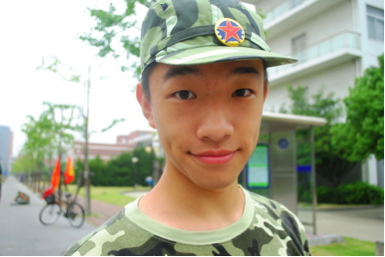
\includegraphics[scale=1]{lmt}
	\caption{Sam}
\end{figure}
I`m a senior student whose major is Electrical and Computer Engineering in Shanghai Jiao Tong University. I am going to study Computer Engineering in Europe. I used to be a good photographer of the Joint Institute, and an excellent goal keeper of institute`s soccer team. I love driving, once drove my Mustang from Michigan all the way to Miami with another friend in two days. And I have attended Zero-Gravity flight in Las Vegas, which was a unique experience. I pace to higher goals will never stop.
\pagebreak
\subsection{Sasha Sheng}
\begin{figure}[H]
	\centering
	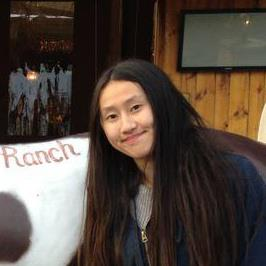
\includegraphics[scale=1]{Profile}
	\caption{Sasha}
\end{figure}
I am Sasha. I am a ME student at JI, and CS student at UM. I love tautology. I love philosophy. I love programming. I love books, music, movies. I will love them until one day I won`t. Hmmm, I have to say sorry to you. Because no matter how much I want to, I can`t give you a more detailed self description. To know the reason, read this: http://www.sashasheng.com/my-journey-on-self-discovery
\pagebreak
\subsection{Christina Yan}
\begin{figure}[H]
	\centering
	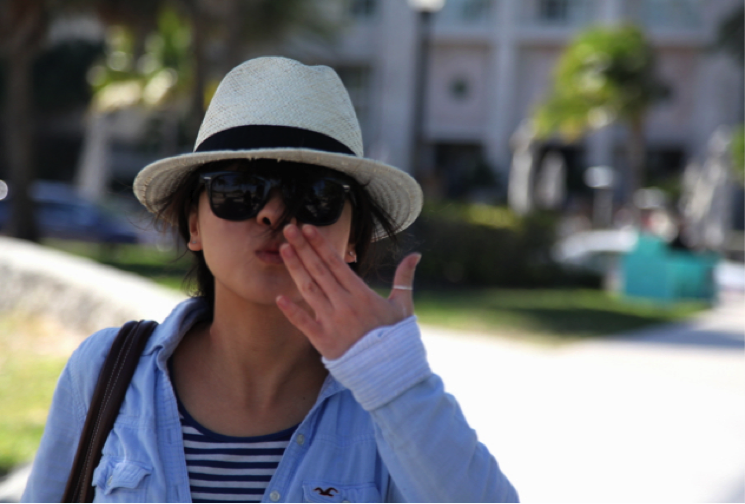
\includegraphics[scale=1]{Christina}
	\caption{Christina}
\end{figure}
I am Christina, a senior student with a major in ECE at SJTU and Architecture at U of M. I spent first two years at engineering and finally found out this was not what I want to do. I transfer to architecture in America and fortunately I love what I am doing there. I have always been grateful that I still have the passion to change the world, not in a technical way any more but in an aesthetical way instead. Maybe it is also a good choice to be a female architect with the programming background in the future. Maybe I also could be a yoga coach someday and doing meditation in India while my friends are all programming. Maybe that is also what god wants to teach me, just follow your inner heart and try your best, life will finally bring you to a wonderland.
\pagebreak
\subsection{Siyuan Zhang}
\begin{figure}[H]
	\centering
	
\includegraphics[scale=0.08]{zsy}
	\caption{Siyuan Zhang}
\end{figure}
I am an Electrical and Computer Engineering major here at Joint Institute, and have got a bachelor`s degree in Computer Engineering at University of Michigan. After graduating I will go to Stanford for Master`s degree in Computer Science. My home town is Beijing, and I`ve been going to college at Shanghai, China and Michigan, U.S.A. While I often miss my home town, I`ve also become used to being in unfamiliar places and travelling in a way. I look forward to life in California for the next few years, and I enjoy this summer during which I am in my motherland and can go home more frequently.

Apart from doing school work, I`ve always enjoyed sports. Basketball is my favourite. I have spent quite a lot of time on basketball, which has become an important part of my life. It feels like we`ve known each other for many years, and we will be friends for a life time. I also like music and dancing. I`m a starter in doing a kind of old-school street dancing called locking dance. Unfortunately it`s known by few people around me. I think the reason is that it is too old-school for today`s United States, and in China it just never has been widely known. However, I`m seeing more events happening in Shanghai, China or even in Asia as a whole about the dancing styles that I like. Frankly speaking I think it`s far better than the so-called "modern dance styles" that appears on television these days. I believe that good things never fade away, sometimes people just don`t know them. I`m excited to see new developments of these old dance styles and the flourishing of them.
\pagebreak
\subsection{Wang Zi}
\begin{figure}[H]
	\centering
	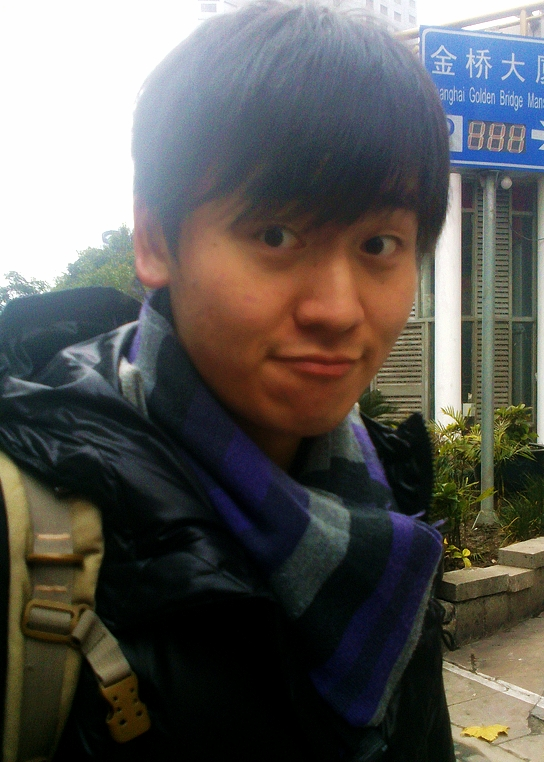
\includegraphics[scale=0.5]{W.jpg}
	\caption{Wang Zi}
\end{figure}
I am Wang Zi, a senior student from UMJI-SJTU. My major is Electronic and Computer Engineering. I get 2011-2012 SJTU Outstanding Scholarship in my third year of University. During my college, I take part in several school projects, concerning about electronic circuit designing, processor coding and mobile software programming. I am interested in Internet and mobile, both software and hardware. Besides of my schoolwork, I am fond of taking social activities both in and outside of SJTU. I work as a school Jing Jing Ambassador whose duty is to Receive various companies such as Deloitte and Xiaomi and help to hold their recruitment fair. I am leader of SK Sunny International Volunteer Program, during which time I lead a team of 15 students from SJTU to serve for the old as volunteers. 
\pagebreak
\bibliographystyle{plain}
\bibliography{DR1}
\pagebreak
\begin{landscape}
\section{Appendix - Gantt Chart}
\begin{figure}[H]
    	\advance\leftskip-1.5cm
	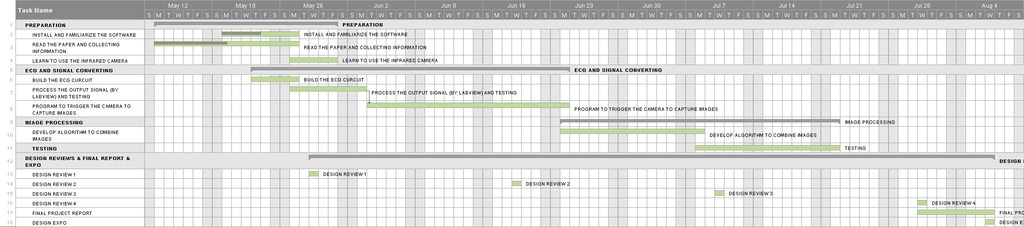
\includegraphics[scale=0.7]{GANTT}
	\caption{Gantt Chart}
\end{figure}
\end{landscape}
\end{document}
